\documentclass[oneside,12pt,letterpaper]{article}

% Imports and Definitions
%% Packages
\usepackage{amsmath}
\usepackage{amsfonts}
\usepackage{amssymb}
\usepackage{amsthm}
\usepackage{arydshln}
\usepackage{color}
\usepackage{extramarks}
\usepackage{fancyhdr}
\usepackage{float}
\usepackage[margin=1in]{geometry}
\usepackage{graphicx}
\usepackage{listings}
\usepackage{multicol}
\usepackage{setspace}
\usepackage{subcaption}
\usepackage{textcomp}
\usepackage{url}
\usepackage{xspace}
\usepackage{mathtools}

%% Commands
%%% Metadata
\newcommand{\metaTitle}{Comprehensive Exam}
\newcommand{\metaDueDate}{November 24, 2020}
\newcommand{\metaDueTime}{04:00 PM}
\newcommand{\metaSchool}{IUPUI}
\newcommand{\metaClass}{STAT 52400}
\newcommand{\metaDepartment}{Statistics Department}
\newcommand{\metaAuthorName}{Ross Grinvalds}

%%% Aliases
\newcommand{\Bias}{\mathrm{Bias}}
\newcommand{\Cov}{\mathrm{Cov}}
\newcommand{\dd}[1]{\frac{\mathrm{d}}{\mathrm{d}x} (#1)}
\newcommand{\dx}{\mathrm{d}x}
\newcommand{\E}{\mathrm{E}}
\newcommand{\m}[1]{\begin{bmatrix*}[r]#1\end{bmatrix*}}
\newcommand{\md}[1]{\begin{vmatrix*}#1\end{vmatrix*}}
\newcommand{\mf}[1]{\mathrm{\bf{#1}}}
\newcommand{\p}[1]{\begin{pmatrix}#1\end{pmatrix}} 
\newcommand{\pdd}[2]{\frac{\partial}{\partial #1} (#2)}
\newcommand{\solution}{\textbf{\large Solution}}
\newcommand{\T}{\intercal}
\newcommand{\Var}{\mathrm{Var}}

%%% Math Functions
\makeatletter
\newsavebox{\mybox}\newsavebox{\mysim}
\newcommand{\distras}[1]{%
  \savebox{\mybox}{\hbox{\kern3pt$\scriptstyle#1$\kern3pt}}%
  \savebox{\mysim}{\hbox{$\sim$}}%
  \mathbin{\overset{#1}{\kern\z@\resizebox{\wd\mybox}{\ht\mysim}{$\sim$}}}%
}
\makeatother

\newcommand{\indep}{\perp \!\!\! \perp}

%% Environments
%%% R Code
\newcommand{\ri}[1]{\lstinline{#1}}  %% Short for 'R inline'

\lstnewenvironment{rc}[1][]{
	\lstset{commentstyle=\color{red}, keywordstyle=\color{black}, showstringspaces=true, language=R, basicstyle=\ttfamily\tiny}
}{}
\lstset{language=R}


% Settings
%% Document-wide
\pagestyle{fancy}

%% Header and Footer
\setlength{\headheight}{15pt}
\lhead{\metaAuthorName}
\chead{\metaSchool\ \metaClass:\ \metaTitle}
\rhead{\metaDepartment}
\cfoot{\thepage}

%% Title Page
\title{
	\vspace{1in}
	\textmd{\textbf{\metaSchool\ \metaClass:\ \metaTitle}}\\
	\normalsize\vspace{0.1in}\small{Due\ by\ \metaDueDate\ at \metaDueTime}\\
	\vspace{6in}
}
\author{\metaAuthorName}
\date{}


\begin{document}
\maketitle

\section*{Problem 1}
Given a covariate matrix: $$\mathbf{\Sigma} = \m{3&-3&0\\-3&12&0\\0&0&6}$$
\begin{enumerate}
\item[\bf{a)}]
	To obtain the correlation matrix, let: $$\mf{V}=diag(\mathbf{\Sigma})=\m{3&0&0\\0&12&0\\0&0&6}$$ Then:
	\begin{align*}
		\m{\rho_{ij}}_{i \times j} &= \mf{V}^{-\frac{1}{2}} \mathbf{\Sigma} \mf{V}^{-\frac{1}{2}} \\
									&= \m{1&-0.5&0\\-0.5&1&0\\0&0&1}
	\end{align*}

\item[\bf{b)}]
	If two of the three eigenvalues of the correlation matrix were to be $1.5$ and $1.0$, the remaining eigenvalue can be identified given the following relationship: $$\sum_{i=1}^3\lambda_i=\sum_{i=1}^3\rho_{ii}=3 \implies \lambda_3 = 0.5$$ The third eigenvector, $\vec{e}_3$ can be identified by solving the following system of equations: $$\m{1-0.5&-0.5&0\\-0.5&1-0.5&0\\0&0&1-0.5} \m{e_1\\e_2\\e_3} = \m{0\\0\\0} \implies e_3 = 0,\ e_1 = e_2$$ Therefore, $\vec{e}_3^{\intercal}= \m{\frac{\sqrt{2}}{2}&\frac{\sqrt{2}}{2}&0}$. This leads to the spectral decomposition of the correlation matrix as follows: $$\m{\rho_{ij}}_{i \times j} = \mf{P} \mathbf{\Lambda} \mf{P}' = \m{0.707&0&0.707\\-0.707&0&0.707\\0&1&0} \m{1.5&0&0\\0&1.0&0\\0&0&0.5} \m{0.707&-0.707&0\\0&0&1\\0.707&0.707&0}$$

\item[\bf{c)}]
	The determinant of the matrix $\mathbf{\Sigma}$ is an abstraction of the volume of the transformation that occurs when a vector is transformed by that matrix. It has the following relationship with respect to the eigenvalues of the matrix: $$det(\mathbf{\Sigma}) =\prod_{i=1}^3\lambda_i=12.908\cdot6\cdot2.092=162$$ The trace of a matrix is the sum of its diagonal elements. It has the following relationship with respect to the eigenvalues of the matrix: $$trace(\mathbf{\Sigma})=\sum_{i=1}^3\sigma_{ii}=\sum_{i=1}^3\lambda_i = 12.908 + 6 + 2.092 = 21$$ In the case where the matrix is diagonal, the eigenvalues are the diagonal elements of that matrix.

\item[\bf{d)}]
	Given $\lambda_1 =12.9$ and $\vec{e}_1^{\intercal} = \m{0.29&-0.96&0}$. The eigenvalues and eigenvectors can be calculated by the characteristic equation of $\mathbf{\Sigma}$: $$\md{\mathbf{\Sigma} - \vec{\lambda}\cdot\mathbf{I}_3} = (6 - \lambda)(\lambda^2 - 15\cdot\lambda + 27) \implies \lambda_2 = 6$$ The second eigenvector is computed by the following system of equations: $$\m{-3&-3&0\\-3&6&0\\0&0&0} \m{e_1\\e_2\\e_3} = \m{0\\0\\0} \implies e_3 = 1,\ e_1 = e_2 = 0 \implies \vec{e}_2=\m{0\\0\\1}$$ Utilizing the relationship between the eigenvalues and trace of a matrix, $\lambda_3 = 21 - 12.9 - 6 = 2.1$. The corresponding eigenvector can be found using the properties of an orthogonal matrix, $\mf{P}$. The column vectors of any orthogonal matrix satisfy $\vec{p}_i^{\intercal}\vec{p}_j = 0$ if $i \neq j$ and $\vec{p}_i^{\intercal}\vec{p}_j = 1$ for $i = j$. Then, the last eigenvector can be obtained by solving the following system of equations: $$\m{0.29&-0.96&0\\0&0&1} \m{e_1\\e_2\\e_3} = \m{0\\0\\0} \implies e_1 = 0.96,\ e_2 = 0.29,\ e_3 = 0 \implies \vec{e}_3=\m{0.96\\0.29\\0}$$ 

\item[\bf{e)}]
	The spectral decomposition of $\mathbf{\Sigma}$ is:
	\begin{align*}
		\mathbf{\Sigma} &= \mf{P} \mathbf{\Lambda} \mf{P}'\\
										&= \m{0.29&0&0.96\\-0.96&0&0.29\\0&1&0} \m{12.9&0&0\\0&6&0\\0&0&2.1} \m{0.29&-0.96&0\\0&0&1\\0.96&0.29&0}
	\end{align*}	
	The spectral decomposition of $\mathbf{\Sigma}^{-1}$ is thus:
	\begin{align*}
		\mathbf{\Sigma} &= \mf{P} \mathbf{\Lambda}^{-1} \mf{P}' \\
										&= \mf{P} \m{\frac{1}{12.9}&0&0\\0&\frac{1}{6}&0\\0&0&\frac{1}{2.1}} \mf{P}'
	\end{align*}	
	Similarly, for $\mathbf{\Sigma}^{\frac{1}{2}}$:
	\begin{align*}
		\mathbf{\Sigma} &= \mf{P} \mathbf{\Lambda}^{\frac{1}{2}} \mf{P}' \\
										&= \mf{P} \m{\sqrt{12.9}&0&0\\0&\sqrt{6}&0\\0&0&\sqrt{2.1}} \mf{P}'
	\end{align*}	

\end{enumerate}

\newpage
\section*{Problem 2}
$$\vec{X} = \m{X_1\\X_2\\X_3} \distras{} N_3\p{\m{0\\-1\\2},\ \m{2&-2&1\\-2&5&-2\\1&-2&1}}$$
\begin{enumerate}
\item[\bf{a)}]
	Let:$$\vec{Y} = \p{X_1-X_3\\X_2-X_3}=\mf{A}\vec{X},\ \mf{A} = \m{1&0&-1\\0&1&-1}$$ To identify the distribution of $\vec{Y}$, utilize the properties of combinations of normal random variables: $$\vec{Y} \distras{} N_2\p{\mf{A} \vec{\mu}_X,\ \mf{A} \mathbf{\Sigma} \mf{A}'}$$ Compute the relevant components: $$\mf{A} \vec{\mu}_X = \m{-2\\-3},\ \mf{A} \mathbf{\Sigma} \mf{A}' = \m{1&0\\0&10}$$ Therefore: $$\vec{Y} \distras{} N_2\p{\m{-2\\-3},\ \m{1&0\\0&10}}$$

\item[\bf{b)}]
	In order to ascertain whether $X_1+\frac{1}{2}X_2$ is independent of $X_3$, simply obtain the joint distribution as done in part $\bf{a)}$, now using the matrix: $$\mf{A} = \m{1&\frac{1}{2}&0\\0&0&1}$$ The matrix obtained from this transformation is: $$\vec{Y} = \mf{A} \vec{X} \distras{} N_2\p{\m{-\frac{1}{2}\\2},\ \m{\frac{5}{4}&0\\0&1}}$$ Because ${\sigma_Y}_{12} = 0$ and because each of these variables are distributed as jointly normal, the proposed linear combination is in fact independent.

\item[\bf{c)}]
	A vector $\vec{a}$ such that $X_1$ is independent of $\vec{a}^{\intercal} \m{X_2\\X_3}$ by solving the transformation of the covariance matrix as follows: $$\mf{A}=\m{1&0&0\\0&a_1&a_2},\ \mf{A} \mathbf{\Sigma} \mf{A}' = \m{2&-2a_1+a_2\\-2a_1+a_2&5a_1^2-4a_1a_2+a_2^2}$$ Thus, $X_1$ is independent of $\vec{a}^{\intercal} \m{X_2\\X_3}$ IFF $-2a_1 + a_2 = 0$. Let $a_1 = 1$. Then $a_2 = 2$. Therefore: $$\vec{a} = \m{1\\2} \implies \vec{Y} = \mf{A} \vec{X} \distras{} N_2\p{\m{0\\3},\ \m{2&0\\0&1}}$$

\item[\bf{d)}]
	The conditional distribution of $Y = X_1 | X_2 = x_2,\ X_3 = x_3$ evaluated at $(x_2,\ x_3) = (-1,\ 2)$ can be obtained by partitioning $\vec{X}$ as: $$\vec{X} = \m{X_1 \\ \hline X_2 \\ X_3} = \m{X^{(1)}\\ X^{(2)}},\ \newcommand*{\temp}{\multicolumn{1}{r|}{}} \mathbf{\Sigma} = \left[\begin{array}{cccc} 2 & \temp & -2 & 1 \\ \cline{1-4} -2 & \temp & 5 & 1 \\ 1 & \temp & -2 & 1 \end{array}\right] = \m{\Sigma_{11} & \Sigma_{12} \\ \Sigma_{21} & \Sigma_{22}}$$ Next, compute the conditional mean and variance:
	\begin{align*}
		\E[Y] &= \mu_{X_1} + \m{\Sigma_{12}\Sigma_{22}^{-1}}_{11}(x_2 - \mu_{X_2}) + \m{\Sigma_{12}\Sigma_{22}^{-1}}_{12}(x_3 - \mu_{X_3}) \\
					&= 0 + 0 \cdot 0 + 1 \cdot 0 \\
					&= 0 \\
		\\
		\Var[Y] &= \sigma_{11} - \Sigma_{12} \Sigma_{22}^{-1} \Sigma_{21} \\
					&= 2 - \m{-2&1} \m{1&2\\2&5} \m{-2\\1} \\
					&= 1
	\end{align*}
	Therefore, the conditional distribution is $N\p{0, 1}$.

\item[\bf{e)}]
	The outer product of a single centered observation is a Wishart distribution on one degree of freedom.
	$$\vec{x} \distras{} N_3\p{\vec{\mu},\ \mathbf{\Sigma}}$$
	$$\vec{x} - \vec{\mu} \distras{} N_3\p{\vec{0},\ \mathbf{\Sigma}}$$
	$$\p{\vec{x} - \vec{\mu}}\p{\vec{x} - \vec{\mu}}^{\intercal} = \mathbf{\Sigma} \distras{} W_{p=3}\p{\mathbf{\Sigma},\ n=1}$$

\end{enumerate}

\newpage
\section*{Problem 3}
\begin{enumerate}
\item[\bf{i)}]
	$$\bar{\vec{x}}=\frac{1}{n}\sum_{i=1}^nx_i$$
	\begin{align*}
		\E[\bar{\vec{x}}] &= \frac{1}{n} \sum_{i=1}^n \E[\vec{x}_i] \\
										 &= \frac{n}{n} \vec{\mu} \\
										 &= \vec{\mu} \\
		\\
		\Var[\bar{\vec{x}}] &= \frac{1}{n^2} \sum_{i=1}^n \p{\vec{x} - \vec{\mu}}\p{\vec{x} - \vec{\mu}}^{\intercal} \\
												&= \frac{1}{n} \mathbf{\Sigma} \\
		\\
		\therefore \bar{\vec{x}} \distras{} N_p\p{\vec{\mu}, \frac{1}{n} \mathbf{\Sigma}}
	\end{align*}

\item[\bf{ii)}]
	$$(n-1) \mf{S} = \sum_{i=1}^n \p{\vec{x}_i - \bar{\vec{x}}} \p{\vec{x}_i - \bar{\vec{x}}}^{\intercal}$$ But it is known that: $$\p{\vec{x}_i - \bar{\vec{x}}} \p{\vec{x}_i - \bar{\vec{x}}}^{\intercal} \distras{} W_p\p{\mathbf{\Sigma},\ 1}$$ Therefore, the sum of n independent observations leads to: $$\sum_{i=1}^n \p{\vec{x}_i - \bar{\vec{x}}} \p{\vec{x}_i - \bar{\vec{x}}}^{\intercal} \distras{} W_p\p{\mathbf{\Sigma},\ n-1}$$

\item[\bf{iii)}]
	Notice that: $$\p{\vec{x}_i - \bar{\vec{x}}}^{\intercal} \mathbf{\Sigma}^{-1} \p{\vec{x}_i - \bar{\vec{x}}} = \p{\mathbf{\Sigma}^{-\frac{1}{2}}\p{\vec{x}_i - \bar{\vec{x}}}}^{\intercal} \p{\mathbf{\Sigma}^{-\frac{1}{2}}\p{\vec{x}_i - \bar{\vec{x}}}}$$ Let: $$\vec{Y} = \mathbf{\Sigma}^{-\frac{1}{2}}\p{\vec{x}_i - \bar{\vec{x}}} \distras{} N_p\p{\vec{0},\ \mf{I}_p}$$ Then: $$\vec{Y}^{\intercal}\vec{Y} = \sum_{i = 1}^n y_i^2 \distras{} \mathcal{X}^2(p)$$

\item[\bf{iv)}]
	Because $\mf{S} \xrightarrow{P} \mathbf{\mathbf{\Sigma}}$, by Slutsky's Theorem, $\p{\vec{x}_i - \bar{\vec{x}}}^{\intercal} \mf{S}^{-1} \p{\vec{x}_i - \bar{\vec{x}}} \xrightarrow{D} \p{\vec{x}_i - \bar{\vec{x}}}^{\intercal} \mathbf{\Sigma}^{-1} \p{\vec{x}_i - \bar{\vec{x}}}$. Therefore, $\p{\vec{x}_i - \bar{\vec{x}}}^{\intercal} \mf{S}^{-1} \p{\vec{x}_i - \bar{\vec{x}}} \distras{} \mathcal{X}^2(p)$.

\item[\bf{v)}]
	$$ n \p{\bar{\vec{x}} - \vec{\mu}}^{\intercal} \mathbf{\Sigma}^{-1} \p{\bar{\vec{x}} - \vec{\mu}} = \sqrt{n}\p{\mathbf{\Sigma}^{-\frac{1}{2}} \p{\bar{\vec{x}} - \vec{\mu}}}^{\intercal} \sqrt{n}\p{\mathbf{\Sigma}^{-\frac{1}{2}} \p{\bar{\vec{x}} - \vec{\mu}}}$$ Let:
	$$\vec{Y} = \sqrt{n} \p{\bar{\vec{x}} - \vec{\mu}} \distras{} N_p\p{\vec{\mu} - \vec{\mu},\ \frac{\sqrt{n}\sqrt{n}}{n} \mathbf{\Sigma}^{-\frac{1}{2}} \mathbf{\Sigma} \mathbf{\Sigma}^{-\frac{1}{2}}} = N_p\p{\vec{0},\ \mf{I}_p}$$ Therefore, $\vec{Y}^{\intercal} \vec{Y} \distras{} \mathcal{X}^2(p)$.

\item[\bf{vi)}]
	Observe $t^2$: $$t^2=\p{\frac{\p{\bar{x} - \mu}}{\frac{\sigma}{\sqrt{n}}}}^2 \cdot \frac{\frac{\sigma^2}{(n-1)}}{\frac{s^2}{(n-1)}} = \sqrt{n} (\bar{x} - \mu) s^{-2} \sqrt{n} (\bar{x} - \mu) \distras{} F_{1, n-1}$$ Extending this relationship to the multivariate form: $$(n-1) \sqrt{n}\p{\bar{\vec{x}} - \vec{\mu}}^{\intercal} \p{(n-1) \mf{S}}^{-1} \sqrt{n}\p{\bar{\vec{x}} - \vec{\mu}} = T^2$$ Note that $$\sqrt{n}\p{\bar{\vec{x}} - \vec{\mu}} \distras{} N_p\p{\vec{0}, \mathbf{\Sigma}},\ (n-1)\mf{S} \distras{} W_p\p{\mathbf{\Sigma},\ n-1}$$ It follows that $T^2 \distras{} \frac{p(n-1)}{(n-p)}F_{p, n-p}$

\item[\bf{vii)}]
	The statistic defined in $\bf{3.vi)}$ is Hotelling's $T^2$ statistic and can be used to test the following set of hypotheses:$$H_0: \vec{\mu} =\vec{\mu}_0,\ H_a: \vec{\mu} \neq \vec{\mu}_0$$ The test is conducted by first calculating the sample mean vector and then calculating the statistical distance between the sample mean vector and the mean vector under the null hypothesis. $$T^2 = n \p{\bar{\vec{x}} - \vec{\mu}_0} \mf{S} ^{-1} \p{\bar{\vec{x}} - \vec{\mu}_0} \distras{} \frac{p(n-1)}{(n-p)}F_{p, n-p}$$

\item[\bf{viii)}]
The $T^2$ test statistic is compared against the critical value of the $F$ distribution with $p$ and $n-p$ degrees of freedom for the numerator and denominator, respectively. Letting $\alpha$ to be the risk of committing a Type I error, the null hypothesis is rejected if $T^2$ falls in the rejection region defined by: $$T^2 > \frac{p(n-1)}{(n-p)} F_{p, n-p}^*(1 - \alpha)$$ This test is equivalent to calculating $P\p{F_{p, n-p} > T^2}$ and rejecting the null hypothesis if the calculated p-value is less than $\alpha$.

\end{enumerate}

\newpage
\section*{Problem 4}
This question focuses on one variety of the famous iris dataset, given in $petal.txt$. The measurements for this particular variety of iris include Septal Length (Length) and Septal Width (Width). The dataset contains $n = 50$ observations.

\begin{enumerate}
\item[\bf{a)}] 
	The first goal is to identify any potential outliers in the dataset and remove them before proceeding with the analysis. In order to identify outliers, first, an inspection of the univariate distributions was performed to see if there were any potentially extreme values. This was done via boxplots for both Length and Width. Potential outliers were identified on the boxplot if the absolute value of the observation exceeds the criterion of $1.5 \times IQR$. The potential univariate outliers were thus $16$ and $42$.
	\begin{center}
		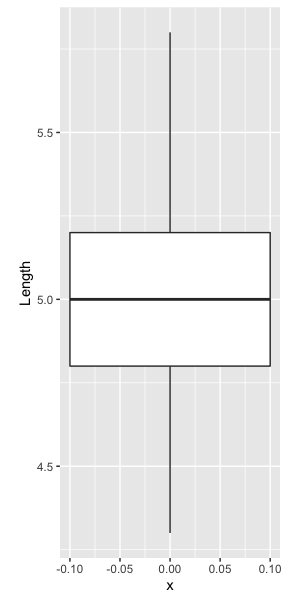
\includegraphics[width=1.5in]{plot_4_a_L_boxplot.png}
		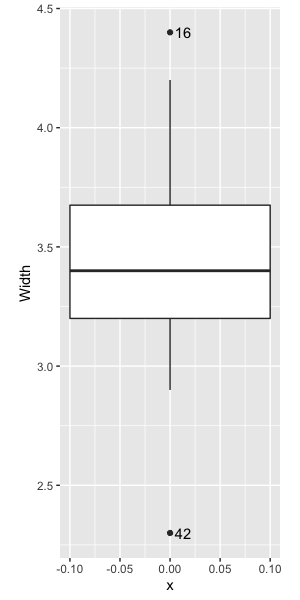
\includegraphics[width=1.5in]{plot_4_a_W_boxplot.png}
	\end{center}
	Standardized values for Length and Width were obtained, and all values exceeding two standard deviations in either the Length or Width measurement were identified. Note that none of the observations exceed an absolute standard deviation of three.
		\begin{rc}
	# A tibble: 5 x 4
		Length std_Length Width std_Width
		 <dbl>      <dbl> <dbl>     <dbl>
	1    4.3      -2.00   3       -1.13
	2    5.8       2.25   4        1.51
	3    5.7       1.97   4.4      2.56
	4    5.5       1.40   4.2      2.04
	5    4.5      -1.44   2.3     -2.98
	\end{rc}
	The bivariate spread of the data is next considered. All generalized squared distances of the observations, calculated as $\p{\vec{x}_i - \bar{\vec{x}}}^{\intercal}\mf{S}^{-1}\p{\vec{x}_i - \bar{\vec{x}}}$, were compared to the critical value of a $\mathcal{X}_2^2(0.99)=9.210$. Shown in the plot below, only observation $42$ exceeded the critical value. For the remainder of the analysis, only observation $42$ will marked as an outlier and removed for consideration.
	\begin{center}
		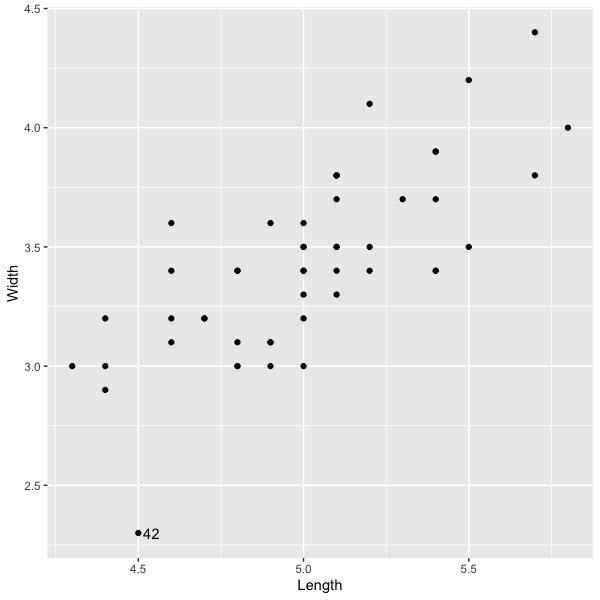
\includegraphics[width=3in]{plot_4_a_LW.png}
	\end{center}

\item[\bf{b)}]
	The assumption of multivariate normality of the Septal Length and Septal Width is next considered. A univariate analysis of normality for both Length and Width suggest roughly normal characteristics. This is assessed via histograms, which measure the shape of the univariate distribution, and quantile-quantile plots, in which linearity (correlation with the theoretical quantiles) implies normality. It is clear that there may be a problem with the normality assumption for Width based on the plots. In addition to the visual analysis, two normality tests were performed in R, the Wilks-Shapiro test and the correlation quantile test. The null hypothesis of all of these tests is that the data are normally distributed. In all four cases, the sample data does not provide evidence to the contrary of the null hypothesis given a risk of committing a Type I error to be $\alpha = 0.05$. However, were a slightly more relaxed $\alpha$, say $\alpha = 0.10$, selected, both tests would fail for Width.
	\begin{center}
		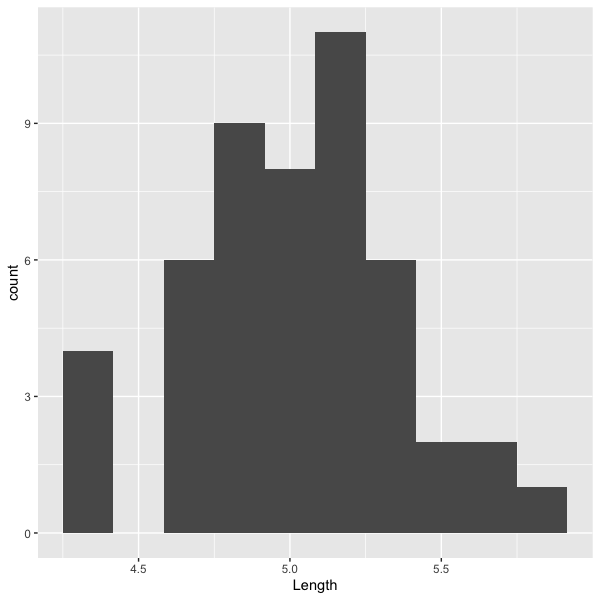
\includegraphics[width=3in]{plot_4_b_L_hist.png}
		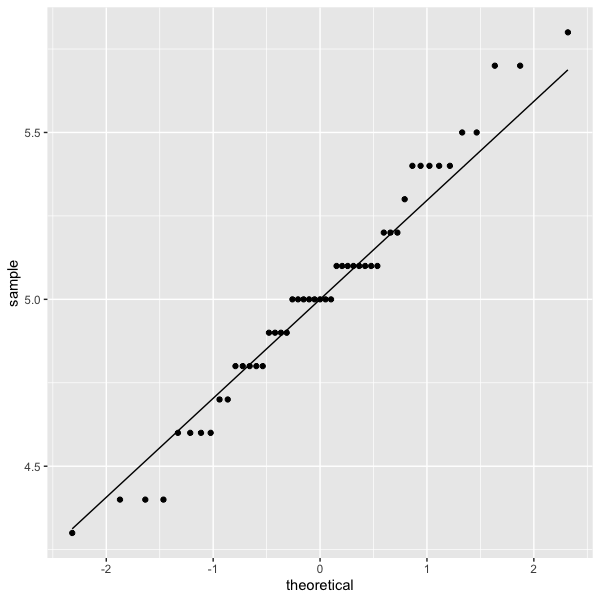
\includegraphics[width=3in]{plot_4_b_L_qq.png}
		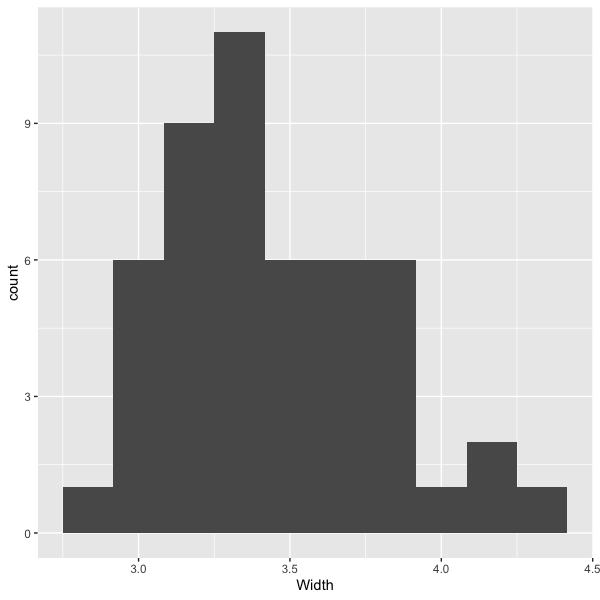
\includegraphics[width=3in]{plot_4_b_W_hist.png}
		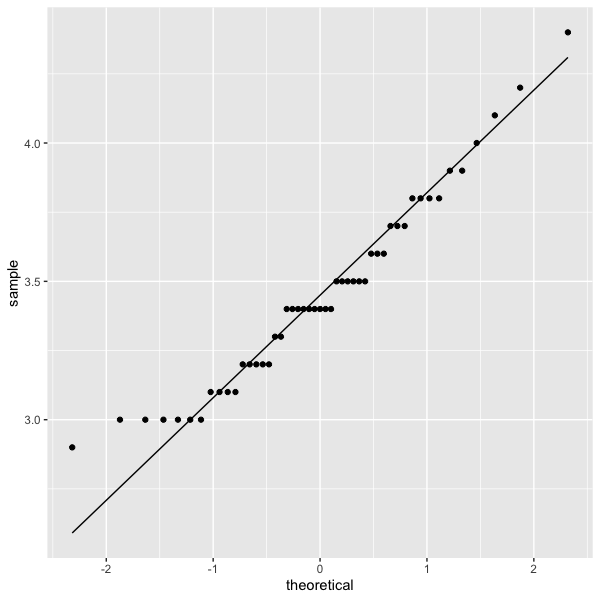
\includegraphics[width=3in]{plot_4_b_W_qq.png}
	\end{center}
	Although by the assumed $\alpha$, all normality tests formally passed, it is worth considering whether or not a transformation on Width will help improve its normality. For both Length and Width, univariate Box-Cox likelihood curves are presented. In the case for Length, it is clear that the the untransformed data ($\lambda_1 = 1$) are adequate. However, for Width, the univariate Box-Cox transformation suggests a transformation somewhere in the range of $-2 < \lambda_2 < -1$. A multivariate Box-Cox analysis suggests that a suitable transformation is to select $\lambda_2 = -1.25$ for the transformation of Width. A contour plot of the multivariate Box-Cox analysis shows how a bivariate set of $\vec{\lambda}$ may be selected.
	\begin{center}
		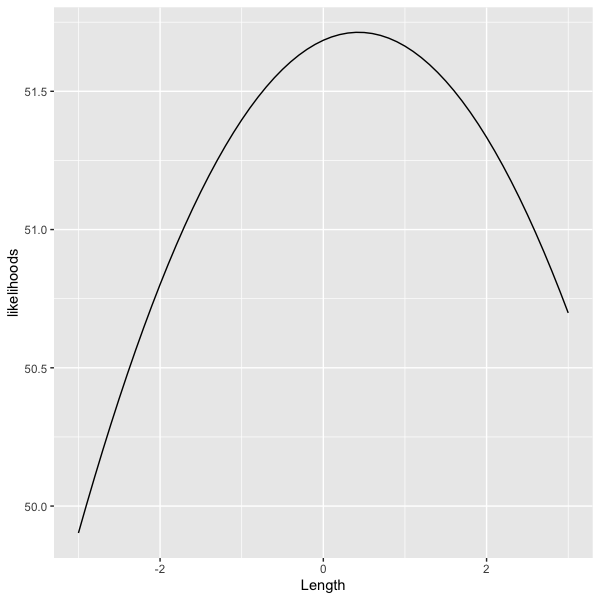
\includegraphics[width=3in]{plot_4_b_L_bxcx.png}
		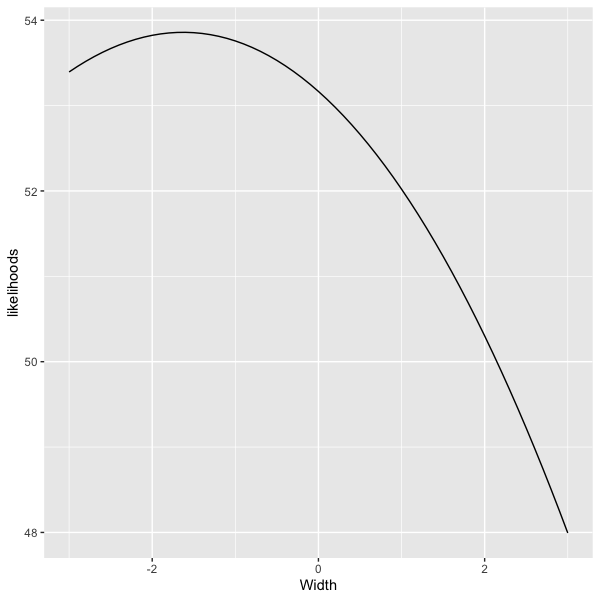
\includegraphics[width=3in]{plot_4_b_W_bxcx.png}
	\end{center}
	\begin{center}
		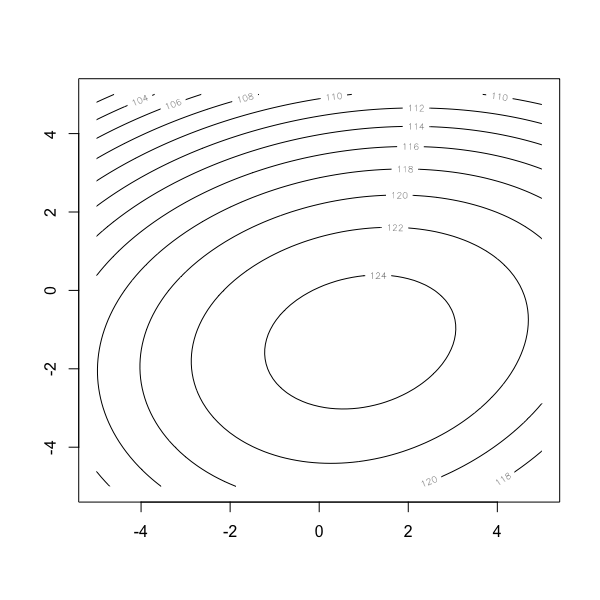
\includegraphics[width=3in]{plot_4_b_LW_bxcx.png}
	\end{center}

\item[\bf{c)}]
	The $95\%$ confidence region for the joint distribution of Length and Width is formed with respect to the critical distribution of the appropriate Hotelling $T^2$ distribution. With $n = 49$ observations on $p = 2$ variables, the confidence region for the population mean vector, $\vec{\mu}$ is given by: $$ 49 \p{\bar{\vec{x}}-\vec{\mu}}^{\intercal} \mf{S}^{-1} \p{\bar{\vec{x}}-\vec{\mu}} < \frac{2\cdot48}{47} F_{2,47}^*(1-\alpha) = 6.526$$ Where: $$\bar{\vec{x}} = \m{5.016 \\ 3.451},\ \mf{S} = \m{0.121 & 0.089 \\ 0.089 & 0.119}$$

\item[\bf{d)}]
	The confidence region above defines an ellipse in two dimensions. The direction of the axes of this ellipse are the eigenvectors of the covariance matrix. The length of the axes is determined by the specified level $\alpha$. In general, the scaling of the ellipse's axes can be determined by: $$\sqrt{\lambda_i} \cdot \sqrt{\frac{p(n-1)}{n(n-p)}F_{p, n-p}^*(1-\alpha)}=\sqrt{\lambda_i} \cdot 0.365$$ Where $\lambda_i$ corresponds to the associated eigenvector $\vec{e}_i$. The confidence region defined in part $\bf{c)}$ is drawn on the scatterplot of the data along with two sets of univariate confidence intervals for Length and Width. The wider of the confidence intervals are the $T^2$ intervals that utilize the same distribution specified in part $\bf{c)}$. These can be thought of as the `shadows' of the confidence ellipse on the axes. The narrower of the confidence intervals are simultaneous Bonferroni confidence intervals, which do not take into consideration the covariance between Length and Width. The lower and upper limits of both sets of these intervals, as calculated in R, are provided below the plot.
	\begin{center}
		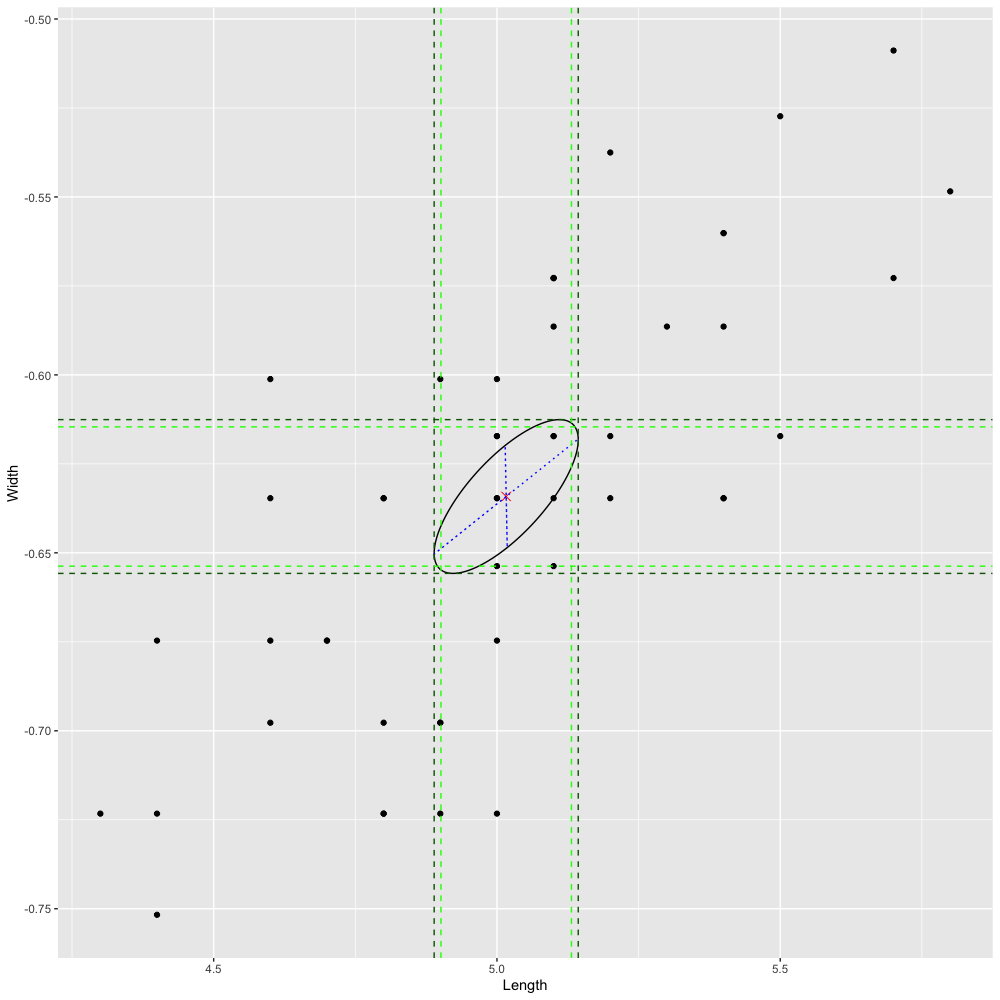
\includegraphics[width=6in]{plot_4_d_conf.png}
	\end{center}
	\begin{rc}
	> CIT2 # T^2 Confidence Intervals
						LCL        UCL
	X1  4.8891733  5.1434798
	X2 -0.6557806 -0.6125677
	> CIBF # Bonferroni Confidence Intervals
						LCL        UCL
	X1  4.9011548  5.1314983
	X2 -0.6537446 -0.6146037
	\end{rc}

\end{enumerate}

\newpage
\section*{Problem 5}
\begin{enumerate}
\item[\bf{a)}]
	``\textit{Any linear combination of normal random variables is still normal.}" This statement is false. A linear combination of normal variables is not guaranteed to be normally distributed. A counterexample presents a proof by contradiction. Let $X \distras{} N\p{0,\ 1}$ and let $Y = -X \implies Y \distras{} N\p{0,\ 1}$. But, $\sigma_{XY} = -1 \implies \mathbf{\Sigma}_{XY} = \m{1&-1\\-1&1}$. The eigenvalues of this covariance matrix are $\lambda_1 = 2$ and $\lambda_2 = 0$. This implies that $\mathbf{\Sigma}_{XY}$ is not a positive definite matrix. But this is a contradiction, because the covariance matrix of any multivariate normal distribution is positive definite. This completes the proof.

\item[\bf{b)}]
	``\textit{If the covariance between two normal random variables is $0$, then the two normal random variables are independent.}" This statement is also false. Zero covariance between two random normal variables is not sufficient for making this conclusion. As a counterexample, let $X \distras{} N\p{0,\ 1}$, let $c > 0$, and define $Y$ as follows: $$Y = \left\{ \begin{array}{cl} X & if \md{X} \leq c \\ -X & if \md{X} > c \end{array} \right.$$ Clearly, $Y \distras{} N\p{0,\ 1}$, however, the covariance between $X$ and $Y$ changes with respect to the selected value of $c$. As $c \xrightarrow{} 0,\ \sigma_{XY} \xrightarrow{} -1$. Similarly, as $c \xrightarrow{} \infty,\ \sigma_{XY} \xrightarrow{} 1$. Then, by the median value theorem, $\exists\ c:\ \sigma_{XY} = 0$. However, $Y$ is dependent on $X$ by definition. Thus the proof is complete.

\end{enumerate}


\end{document}
